\documentclass[a4paper]{article}
\usepackage{amsfonts}
\usepackage{amsmath}
\usepackage{amssymb}
\usepackage{graphicx}     

\newcommand{\Bgtan}{\operatorname{Bgtan}}
\newcommand{\Bgsin}{\operatorname{Bgsin}}

\begin{document}
  
\noindent \large Auteur: Zaky Souai \\
\noindent \large Studierichting:  Informatica\\
\noindent \large Oefeningenreeks 5D nr. 1.5\\

\bigskip

\normalsize

$\displaystyle f(x)=\dfrac{1}{x^2+1}$ op het interval $[-1,1]$\\

Omdat:

$x^2+1>0 \Rightarrow f(x)>0$\\

Dus de oppervlakte tussen de grafiek en de x-as is:

$A=\displaystyle\int_{-1}^{1}\dfrac{1}{x^2+1}dx$\\

$\displaystyle\int\dfrac{1}{x^2+1}dx=\Bgtan(x)$\\

Dus:\\

$A=\left[\Bgtan(x)\right]_{-1}^{1}$\\

$=\Bgtan(1)-\Bgtan(-1)$\\

$\Rightarrow A=2\Bgtan(1) = \dfrac{\pi}{2}$\\

\begin{figure}[h]
    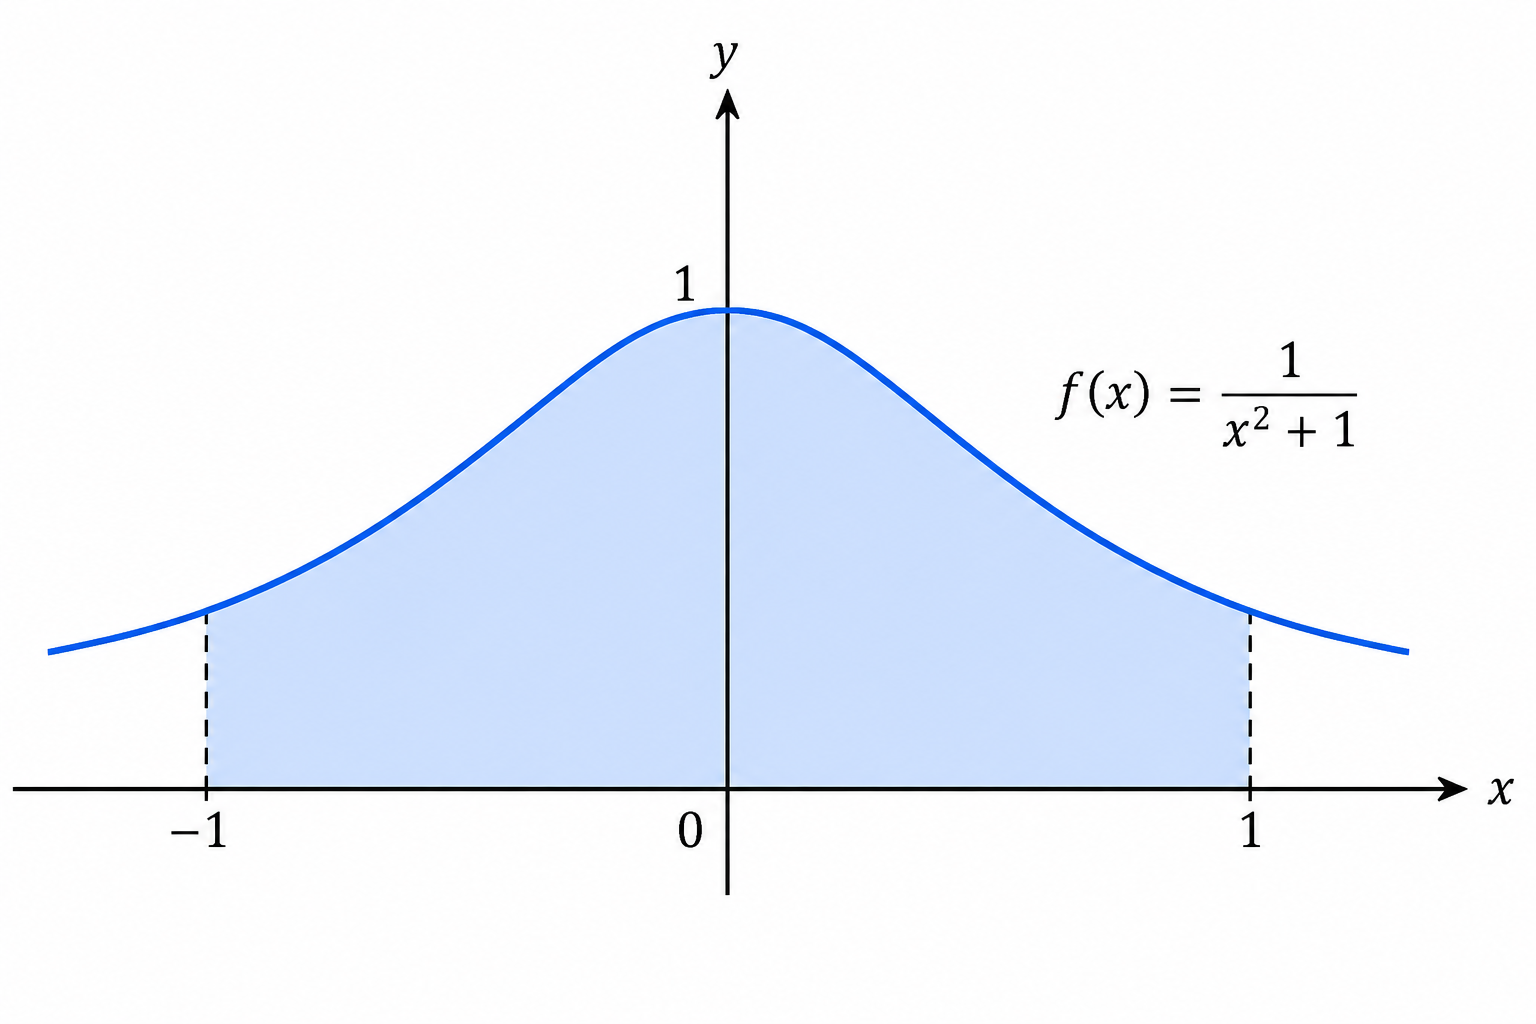
\includegraphics[width=\linewidth]{5D-1.5-zaky.souai.INF.png}\\
\end{figure}

\begin{thebibliography}{999}
%\bibitem{a} Referentie
De tekening werd gegenereerd met AI
\end{thebibliography}
\end{document}